%
% LaTeX-Rahmen f�r Arbeiten am Lehrstuhl Hegering
%
% Nils gentschen Felde, 01/2006
%
% basierend auf Arbeiten von Helmut Reiser, Boris Gruschke,
% Stephen Heilbronner und Harald R�lle
%

\documentclass[a4paper,10pt,twoside,DIV14,BCOR14mm]{scrreprt} 


% !!!!
% !!!! Ausw�hlen der Sprache
% !!!!
\newif\ifLANGDE\LANGDEtrue\newif\ifLANGEN\LANGENfalse   % aktivieren f�r Deutsch
% \newif\ifLANGEN\LANGENtrue\newif\ifLANGDE\LANGDEfalse   % aktivieren f�r Englisch


% !!!!
% !!!! Ausw�hlen der Uni
% !!!!
%\newif\ifTUM\TUMtrue\newif\ifLMU\LMUfalse   % aktivieren f�r TUM
\newif\ifLMU\LMUtrue\newif\ifTUM\TUMfalse   % aktivieren f�r LMU


% !!!!
% !!!! Ausw�hlen des Typs der Ausarbeitung
% !!!!
\newcommand{\typeOfThesis}[0]{Diplomarbeit}
%\newcommand{\typeOfThesis}[0]{Fortgeschrittenenpraktikum}
%\newcommand{\typeOfThesis}[0]{SEP}
%\newcommand{\typeOfThesis}[0]{Studienarbeit}


% !!!!
% !!!! Titel der Arbeit
% !!!!
\newcommand{\titleOfThesisOne}[0]{Titel von SEP/FoPra/DA}
\newcommand{\titleOfThesisTwo}[0]{Titel 2. Zeile}
\newcommand{\titleOfThesisThree}[0]{Titel 3. Zeile}


% !!!!
% !!!! Verfasser der Arbeit
% !!!!
\newcommand{\authorOfThesis}[0]{Vorname Nachname}


% !!!!
% !!!! Aufgabensteller
% !!!!
\newcommand{\aufgabensteller}[0]{Prof. Dr. Dieter Kranzlm\"{u}ller}
%\newcommand{\aufgabensteller}[0]{Prof. Dr. Heinz-Gerd Hegering}
%\newcommand{\aufgabensteller}[0]{Prof. Dr. Claudia Linnhoff-Popien}


% !!!!
% !!!! Betreuer
% !!!!
\newcommand{\betreuerOne}[0]{Vorname Name vom ersten Betreuer}
\newcommand{\betreuerTwo}[0]{Vorname Name vom zweiten Betreuer}
\newcommand{\betreuerThree}[0]{Vorname Name vom dritten Betreuer}


% !!!!
% !!!! Abgabedatum
% !!!!
\newcommand{\abgabeTagZahl}[0]{14}
\newcommand{\abgabeMonatText}[0]{Juli}
\newcommand{\abgabeJahrZahl}[0]{2006}


% !!!!
% !!!! Bibtex files ausw�hlen
% !!!!
% !!!! Variante nur mit lokalen bibfiles (l�uft �berall)
% !!!!
\newcommand{\bibfiles}[0]{bibfile1}
% !!!!
% !!!! Variante inklusive der MNM bibfiles (l�uft nur am Lehrstuhl)
% !!!!
%\newcommand{\bibfiles}[0]{bibfile1,articles,rfcs,internet-drafts,publikationen,diplomarbeiten,dissertationen,fopras,projekte,books,ref,std,in-proceedings,proceedings,ietf-wgs,omg}


% !!!!
% !!!! Ausw�hlen ob Abk�rzungsverzeichnis oder Glossar
% !!!!  Wenn man ein Glossar benutzt, dann sollten Abk�rzungen 
% !!!!  einfach ins Glossar mitaufgenommen werden.
% !!!!
\newif\ifISGLOSS\ISGLOSSfalse   % aktivieren f�r Abk�rzungsverzeichnis
%\newif\ifISGLOSS\ISGLOSStrue    % aktivieren f�r Glossar


%=============================================================================================
% Einbinden der MNM-Definitionen
%=============================================================================================

%
% LaTeX-Rahmen für Arbeiten am Lehrstuhl Hegering
%
% Harald Roelle, 2001,2002
%
% basierend auf Arbeiten von Helmut Reiser, Boris Gruschke und Stephen Heilbronner
%


%=============================================================================================
% Allgemeine Schalter bezueglich des Ausgabeformats
%  MUSS MAN I. A.   N I C H T   ANFASSEN
%=============================================================================================

%
% Check for pdftex
%
%\newif\ifpdf
%\ifx\pdfoutput\undefined
%  \pdffalse % we are not running PDFLaTeX
%\else
%  \pdfoutput=1 % we are running PDFLaTeX
%  \pdftrue
%\fi
\usepackage{ifpdf}


%=============================================================================================
% Einbinden von Packages
%=============================================================================================

% muss ganz am Anfang stehen!
\ifLANGDE%
  \usepackage[british,german]{babel} % => german ist Default zu Beginn (stimmt wirklich!)
  \usepackage{german}        % (neue) deutsche Silbentrennung, ...
  \usepackage{bibgerm}       % deutsche Literaturverzeichnisse
\fi%
\ifLANGEN%
  \usepackage[german,english]{babel} % => english ist Default zu Beginn (stimmt wirklich!)
\fi%

% \usepackage{a4wide}        % weniger Rand  % koenig
\usepackage{url}           % URL's (z.B. in Literatur) schöner formatieren
% \usepackage{tocbibind}     % Literaturverzeichnis erscheint im Inhaltsverz.
\usepackage{supertabular}  % Besonders flexible und grosse Tabellen
\usepackage{makeidx}       % unterstuetzt \makeindex
\usepackage{picins}        % (kleine) Bilder vom Text umfliessen lassen (neu)
% \usepackage{mdwlist}       % für (engere) itemize*-Umgebungen  % koenig
\usepackage{multicol}
% \usepackage{rotating}  % koenig
% \usepackage{epsfig}    % koenig
\usepackage{graphicx}
\usepackage{graphics}
\usepackage{wrapfig}
\usepackage{ifthen}

\usepackage{tikz}
\usepackage{pgfplots}
\usepgfplotslibrary{units}

\usepackage{alltt}

%\usepackage{tabularx} % für Tabellen automagischer Feldbreiten berechnung
%\usepackage{multirow} % für Tabellenfelder, die sich über mehrere Zeilen erstrecken
%\usepackage{subfigure} % um mehrere Abbildungen in einer figure-Umgebung zu strukturieren
%\usepackage{paralist} % für kompakte und nutzerdefinierte itemize und enumerate umgebungen

\ifLANGDE%
  \usepackage[german]{nomencl}       % Abkürzungsverzeichnis
  \ifISGLOSS%
    \renewcommand{\nomname}{Glossar}%
  \else%
    \renewcommand{\nomname}{Abk\"{u}rzungsverzeichnis}%
  \fi%
\fi%
\ifLANGEN%
  \usepackage[english,compatible]{nomencl}       % Abkürzungsverzeichnis
  \ifISGLOSS%
    \renewcommand{\nomname}{Glossary}%
  \else%
    \renewcommand{\nomname}{List of Abbreviations}
  \fi%
\fi%
\renewcommand{\nomlabel}[1]{\textbf{#1}\hfil}%
 
\usepackage{parskip}


%
% Times als Font einstellen
%
\usepackage{rawfonts}
\usepackage{times}


%
% Umlaute direkt im Quellcode
%
% \usepackage[iso]{umlaute}  % koenig

\usepackage[utf8]{inputenc}


%
% Ermöglicht den Pretty-Print der Programmcodes
%
\usepackage{listings}
%\usepackage[breaklines]{listings}
%
% Standards für die Ausgabe der Pretty-Prints !!! SMALL !!!
%
 \lstset{basicstyle=\small\ttfamily, keywordstyle=\bfseries,
  commentstyle=\color{blue}, stringstyle=\itshape,
  extendedchars=true}
% XXXXXXXXXXXXXXXXXXXXXX
%  labelstyle=\tiny\ttfamily, labelstep=2, labelsep=5pt, extendedchars=true}
% numberstyle=\tiny\ttfamily, stepnumber=2, numbersep=5pt, extendedchars=true}


%
% Easy way changing title/section/... appearence
%
\usepackage{titlesec}


%
% muss an dieser Stelle stehen
%
%\usepackage{html}
\usepackage{hyperref}


%
% PDF-Spezifische Angaben
%
\ifpdf
  \pdfcompresslevel=9
  %\usepackage{thumbpdf}  % koenig
  \hypersetup{ a4paper=true,
               plainpages=false,
               pdftex=true,
               hyperindex=true,
               bookmarks=true,
               bookmarksopen=true,
               bookmarksnumbered=true,
               pdfauthor={\authorOfThesis},
               pdftitle={\titleOfThesisOne \titleOfThesisTwo \titleOfThesisThree}
             }
\fi

%
% Rudimentäre Kommentar-Makros
%
\usepackage{color}

\definecolor{fixmecolor}{rgb}{1.0,0.4,0.4}
\definecolor{todocolor}{rgb}{0.4,1.0,0.4}
\definecolor{notecolor}{rgb}{0.4,0.4,1.0}

\newcommand{\fixme}[1]{\textcolor{fixmecolor}{[FIXME: #1]}}
\newcommand{\todo}[1]{\textcolor{todocolor}{[TODO: #1]}}
\newcommand{\note}[1]{\textcolor{notecolor}{[NOTE: #1]}}

%Kommentare für finalen Build ausschalten:
%\newcommand{\fixme}[1]{}
%\newcommand{\todo}[1]{}
%\newcommand{\note}[1]{}

%
% In geralpha-mnm-0.2.bst wird \mnmbiburl als Makro zum Erstellen der URL Links benutzt
% Das hier benutzte \refHTML funltioniert in tex, pdf und html
%
\newcommand{\mnmbiburl}[2]{\refHTML{#1}{#2}}


%=============================================================================================
% Einige Makros
%=============================================================================================

\newcommand{\product}[2][X]{%
  \if#1X%
  \else%
    \index{#1#2}%
  \fi%
  \textsl{#2}%
}

\newcommand{\vendor}[2][X]{%
  \if#1X%
  \else%
    \index{#1#2}%
  \fi%
  \textsf{#2}%
}

\newcommand{\code}[2][X]{%
  \if#1X%
  \else%
    \index{#1#2}%
  \fi%
  \texttt{#2}%
}

\newcommand{\filepath}[2][X]{%
  \if#1X%
  \else%
    \index{#1#2}%
  \fi%
  \texttt{#2}%
}

\newcommand{\texturl}[2][X]{%
  \if#1X%
  \else%
    \index{#1#2}%
  \fi%
  \texttt{#2}%
}


%=============================================================================================
%
% Abkürzungsverzeichnis und Glossar
%

\newcommand{\newAbbrev}[4][X]{%
  \if#1X%
    \index{#3}%
    \index{#4}%
  \else%
    \index{#1#3}%
    \index{#1#4}%
  \fi%
  \nomenclature{#3}{#4}%
  \textbf{#2} (\textbf{#3})%
}%

\newcommand{\listofAbbrevGloss}{%
    \cleardoublepage%
    \ifpdf%
      \pdfbookmark[0]{\nomname}{abkuerungsverzeichnis}%
    \else%
      \addcontentsline{toc}{chapter}{\nomname}%
    \fi%
    \printglossary% % koenig
}

%=============================================================================================
%
% Index
%

\newcommand{\newTerm}[2][X]{%
  \if#1X%
    \index{#2}%
  \else%
    \index{#1#2}%
  \fi%
  \textbf{#2}%
}

\newcommand{\theIndex}[0]{%
  \cleardoublepage%
  \printindex%
}

%=============================================================================================
%
% Quelltext einbinden
%

%
% Umgebung für Listings
%
  \let\verbatim\relax%
  \gdef\wasVerbatimSetupGiven{X}%
  \newcommand{\internalDirtyHackToGetCaption}{}%
  \newcommand{\internalDirtyHackToGetLabel}{}%
  \newcommand{\setupVerbatim}[1]{%
    \renewcommand{\internalDirtyHackToGetCaption}{X}%
    \lstset{language=#1,frame=,basicstyle=,caption={[]},escapechar=}%
    \gdef\wasVerbatimSetupGiven{}%
  }%
  \newcommand{\setupVerbatimBash}{%
    \renewcommand{\internalDirtyHackToGetCaption}{X}%
    \lstset{language=bash,frame=,basicstyle=, caption={[]},escapechar=}%
    \gdef\wasVerbatimSetupGiven{}%
  }%
  \newcommand{\setupVerbatimOut}{%
    \renewcommand{\internalDirtyHackToGetCaption}{X}%
    \lstset{language=,frame=,basicstyle=, caption={[]},escapechar=@}%
    \gdef\wasVerbatimSetupGiven{}%
  }%
  
  \newcommand{\setupVerbatimCaption}[3]{%
    \renewcommand{\internalDirtyHackToGetCaption}{#2}%
    \renewcommand{\internalDirtyHackToGetLabel}{#3}%
    \lstset{language=#1,basicstyle=,captionpos=t,frame=tb,escapechar=}%
    \gdef\wasVerbatimSetupGiven{}%
  }%
  \lstnewenvironment{verbatim}[1][]{%
    \if \wasVerbatimSetupGiven X
      \errmessage{#### No setup command given for new verbatim environment}%
    \fi%
    \gdef\wasVerbatimSetupGiven{X}%
    \if \internalDirtyHackToGetCaption X
      \smallskip
      \lstset{caption={[]}}%
    \else%
      \lstset{caption={\internalDirtyHackToGetCaption},label={listing:\internalDirtyHackToGetLabel}}%
    \fi%
  }{%
  }%


%
% Listing aus File
% {file}{language}
%
\newcommand{\inputListing}[2]{%
  \smallskip
  \lstinputlisting[language=#2,caption={[]}]{#1}%
}%

%
% Listing aus File mit Beschriftung und Begrezungslinien
% {file}{language}{caption}{label}
%
\newcommand{\inputListingCaption}[4]{%
  \lstinputlisting[language=#2,captionpos=t,frame=tb,caption={#3},label={listing:#4}]{#1}%
}%

%
% Umgebung für Beispiele
%
\newenvironment{quoteExample}[0]{%
  \begin{quotation}%
    \noindent%
}{%
  \end{quotation}%
}


%=============================================================================================
%
% Listen
%

%
% Umgebung für Definitionslisten mit festem Einzug
%
\newcommand{\deflabel}[1]{\textbf{#1}}%
\newenvironment{descriptionIndent}[1][2cm]{%
    \begin{list}
      \renewcommand{\makelabel}{\deflabel}%
      %\setlength{\topsep}{0pt}%
      %\setlength{\partopsep}{0pt}%
      %\setlength{\itemsep}{0pt}%
      %\setlength{\parsep}{0pt}%
      \setlength{\leftmargin}{#1}%
      \setlength{\labelwidth}{#1}%
      \setlength{\labelsep}{0.3cm}%
      \addtolength{\labelwidth}{-0.5cm}%
    \end{list}%
}

%=============================================================================================
%
% Referenzen
%

%
% Referenz auf externe URL mit Hyperlink: <text> <URL>
%
\newcommand{\refHTML}[2]{%
    \htmladdnormallink{#1}{#2}%
}


%=============================================================================================
%
% Bilder
%

%
% Bild in einer Spalte
%  <figure_env_args> <inclgraphics_args> <filename> <label> <caption>
%
\newcommand{\includeFigure}[5]{%
  \begin{figure}[#1]%
    \begin{center}%
        % \psfull % koenig
        \includegraphics[#2]{#3}%
        % \psdraft % koenig
        \caption{\label{fig:#4}#5}%
    \end{center}%
  \end{figure}%
}

%
% Bild von Text umflossen
%  <parpic_args> <inclgraphics_args> <filename> <label> <caption>
%
\newcommand{\includeParpic}[5]{%
    \piccaption[#5]{#5 \label{fig:#4}}%
    \parpic[#1]{%
      \includegraphics[#2]{#3}%
    }%
} 

\newcommand{\includeParPic}[6]{%
\begin{wrapfigure}{#1}{#2}%
	\begin{center}%
      \includegraphics[#3]{#4}%
	\end{center}%
	\caption[#6]{#6 \label{fig:#5}}%
\end{wrapfigure}%
}

%
% Abstract der Arbeit
%
\newenvironment{DAabstract}[0]{%
  \newpage%
  \bigskip%
  \thispagestyle{empty}%
  \begin{abstract}%
}{%
  \end{abstract}%
  \thispagestyle{empty}%
  \cleardoublepage%
}%


%
% Wrapper fuer Dokumentanfang
%
\newcommand{\docbegin}[0]{%
  \makeglossary%
  \makeindex%

  \begin{document}%

  %
  % Trennregeln einbinden (MUSS nach begin{document} stehen!)
  %
  %
% der Befehl \hypenation versteht keine Sonderzeichen, also weder ä
% noch "a noch \"a. Wörter die derartige Zeichen enthalten müssen
% direkt im Text getrennt werden, z.B. Wör\-ter
%
\hyphenation{Ma-nage-ment}
\hyphenation{Ma-nage-ment-agent}
\hyphenation{Ma-nage-ment-agent-en}
\hyphenation{Ma-nage-ment-ar-chi-tek-tur}
\hyphenation{Ma-nage-ment-ar-chi-tek-tu-ren} 
\hyphenation{Ma-nage-ment-an-wen-dung}
\hyphenation{Ma-nage-ment-an-wen-dung-en}
\hyphenation{Ma-nage-ment-an-for-der-ung}
\hyphenation{Ma-nage-ment-funk-ti-on}
\hyphenation{Ma-nage-ment-funk-ti-onen}
\hyphenation{Ma-nage-ment-kon-zep-te}
\hyphenation{Ma-nage-ment-res-source}
\hyphenation{Ma-nage-ment-in-for-ma-ti-on}
\hyphenation{Ma-nage-ment-res-sour-cen}
\hyphenation{ma-nage-ment-re-le-vante}
\hyphenation{ma-nage-ment-sy-stem}
\hyphenation{ma-nage-ment-sy-steme}
\hyphenation{Ma-nage-ment-in-stru-men-tie-rung}
\hyphenation{Ma-nage-ment-platt-form}
\hyphenation{Sys-te-men}
\hyphenation{Sys-tem-um-ge-bun-gen}
\hyphenation{Sys-tem-ma-nage-ment}
\hyphenation{DHCP}
\hyphenation{Ma-nage-ment-diszi-plinen}
\hyphenation{System-management-architekturen}
\hyphenation{Verwendungs-nachweise}
\hyphenation{Video-einricht-ungen}
\hyphenation{Res-source}
\hyphenation{Res-sourcen}
\hyphenation{res-sourcen}
\hyphenation{MASA}
\hyphenation{Grund-anwendung}
\hyphenation{Grund-anwendungen}
\hyphenation{Basis-anwendung}
\hyphenation{Core}
\hyphenation{Kom-mu-ni-ka-ti-on}
\hyphenation{De-sign-ent-schei-dung}
\hyphenation{Sprung-ad-res-sen}
\hyphenation{Klas-si-fi-ka-ti-on}
\hyphenation{Schreib-recht}
\hyphenation{Be-nut-zer-zer-ti-fi-kat}
\hyphenation{Bau-stein-ent-wi-ckler}
\hyphenation{ad-mi-ni-stra-ti-ve}

%

  % Titelseiten
  \ifTUM%
    %
% LaTeX-Rahmen f�r Arbeiten am Lehrstuhl Hegering
%
% Harald Roelle, 2001, 2002
% Modified by Nils gentschen Felde, 2006
%
% basierend auf Arbeiten von Helmut Reiser, Boris Gruschke und Stephen Heilbronner
%


%Link im PDF
\ifpdf
  \pdfbookmark[0]{Titel}{Titel}%
\fi

%%%%%%%%%%%%%%%%%%%%%%%%%%%%%%%
% erste Seite

\thispagestyle{empty}

\begin{center}


\includegraphics[width=3cm]{tum-logo}

\vspace{1cm}

{\Huge FAKULT�T F�R INFORMATIK\\[1mm]}
DER TECHNISCHEN UNIVERSIT�T M�NCHEN\\

\vspace{2cm}

{\Large \textbf{\typeOfThesis\ in Informatik}}\\

\vspace{2.0cm}
{\Huge \textbf{\titleOfThesisOne}}\\
\vspace*{3mm}
{\Huge \textbf{\titleOfThesisTwo}}\\
\vspace*{3mm}
{\Huge \textbf{\titleOfThesisThree}}\\

\vspace{1.5cm}

\parbox{1cm}{
  \begin{Large}
    \begin{tabbing}
%      Bearbeiter: \hspace{5mm}
        \authorOfThesis\\[2mm]
%      Aufgabensteller:
%        \>\aufgabensteller\\[2mm]
%      Betreuer: 
%        \>\betreuerOne\\
%        \>\betreuerTwo\\[2mm]
%        \>\betreuerThree\\
%      Abgabetermin: 
%        \> \abgabeTagZahl.~\abgabeMonatText~\abgabeJahrZahl\\
    \end{tabbing}
  \end{Large}
}\\

\vspace{10mm}

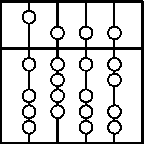
\includegraphics[width=2.4cm]{tum-abakus}

\end{center}

\newpage

%%%%%%%%%%%%%%%%%%%%%%%%%%%%%%%
% zweite Seite

\thispagestyle{empty}
\cleardoublepage 

%%%%%%%%%%%%%%%%%%%%%%%%%%%%%%%
% dritte Seite

\thispagestyle{empty}

\begin{center}


\includegraphics[width=3cm]{tum-logo}

\vspace{1cm}

{\Huge FAKULT�T F�R INFORMATIK\\[1mm]}
DER TECHNISCHEN UNIVERSIT�T M�NCHEN\\

\vspace{2cm}

{\Large \textbf{\typeOfThesis\ in Informatik}}\\

\vspace{2.0cm}
{\Huge \textbf{\titleOfThesisOne}}\\
\vspace*{3mm}
{\Huge \textbf{\titleOfThesisTwo}}\\
\vspace*{3mm}
{\Huge \textbf{\titleOfThesisThree}}\\

\vspace{1.5cm}

\parbox{1cm}{
  \begin{large}
    \begin{tabbing}
      Bearbeiter: \hspace{1cm}
        \=\authorOfThesis\\[2mm]
      Aufgabensteller:
        \>\aufgabensteller\\[2mm]
      Betreuer: 
        \>\betreuerOne\\
        \>\betreuerTwo\\
      Abgabedatum: 
        \> \abgabeTagZahl.~\abgabeMonatText~\abgabeJahrZahl\\
    \end{tabbing}
  \end{large}
}\\

\vspace{5mm}

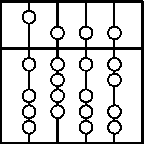
\includegraphics[width=2.4cm]{tum-abakus}

\end{center}
%
  \fi%
  \ifLMU%
    %
% LaTeX-Rahmen für Arbeiten am Lehrstuhl Hegering
%
% Harald Roelle, 2001, 2002
%
% basierend auf Arbeiten von Helmut Reiser, Boris Gruschke und Stephen Heilbronner
%


%Link im PDF
\ifpdf
  \pdfbookmark[0]{Titel}{Titel}%
\fi

%%%%%%%%%%%%%%%%%%%%%%%%%%%%%%%
% erste Seite

\thispagestyle{empty}

\begin{center}

\vspace*{-2cm}

{\Huge INSTITUT FÜR INFORMATIK\\[1mm]}
DER LUDWIG--MAXIMILIANS--UNIVERSITÄT MÜNCHEN\\

\vspace*{1cm}


\includegraphics[width=0.3\textwidth]{lmu_siegel}

\vspace*{2cm}

{\Large \textbf{\typeOfThesis}}\\

\vspace{2.0cm}
{\Huge \textbf{\titleOfThesisOne}}\\
\vspace*{3mm}
{\Huge \textbf{\titleOfThesisTwo}}\\
\vspace*{3mm}
{\Huge \textbf{\titleOfThesisThree}}\\

\vspace{1.5cm}

{\LARGE \authorOfThesis}\\[2mm]
{\LARGE \authorOfThesisOne}\\[2mm]
{\LARGE \authorOfThesisTwo}\\[2mm]

%\vspace{2cm}

%\parbox{1cm}{
%  \begin{large}
%    \begin{tabbing}
%      Aufgabensteller:
%        \=\aufgabensteller\\[2mm]
%      Betreuer: 
%        \>\betreuerOne\\
%        \>\betreuerTwo\\
%        \>\betreuerThree\\[5mm]
%      Abgabetermin: 
%        \> \abgabeTagZahl.~\abgabeMonatText~\abgabeJahrZahl\\
%    \end{tabbing}
%  \end{large}
%}\\

\end{center}

\newpage

%%%%%%%%%%%%%%%%%%%%%%%%%%%%%%%
% zweite Seite

\thispagestyle{empty}
\cleardoublepage 

%%%%%%%%%%%%%%%%%%%%%%%%%%%%%%%
% dritte Seite (Kopie der ersten)

\thispagestyle{empty}

\begin{center}

\vspace*{-2cm}

{\Huge INSTITUT FÜR INFORMATIK\\[1mm]}
DER LUDWIG--MAXIMILIANS--UNIVERSITÄT MÜNCHEN\\

\vspace*{1cm}


\includegraphics[width=0.3\textwidth]{lmu_siegel}

\vspace*{2cm}

{\Large \textbf{\typeOfThesis}}\\

\vspace{2.0cm}
{\Huge \textbf{\titleOfThesisOne}}\\
\vspace*{3mm}
{\Huge \textbf{\titleOfThesisTwo}}\\
\vspace*{3mm}
{\Huge \textbf{\titleOfThesisThree}}\\

\vspace{1.5cm}

{\LARGE \authorOfThesis}\\[2mm]
{\LARGE \authorOfThesisOne}\\[2mm]
{\LARGE \authorOfThesisTwo}\\[2mm]

\vspace{2cm}

\parbox{1cm}{
  \begin{large}
    \begin{tabbing}
      Aufgabensteller:
        \=\aufgabensteller\\[10mm]
      Abgabetermin: 
        \> \abgabeTagZahl.~\abgabeMonatText~\abgabeJahrZahl\\
    \end{tabbing}
  \end{large}
}\\

\end{center}
%
  \fi%
  
  % Erklärung
  %%
% LaTeX-Rahmen f�r Arbeiten am Lehrstuhl Hegering
%
% Harald Roelle, 2001, 2002
%
% basierend auf Arbeiten von Helmut Reiser, Boris Gruschke und Stephen Heilbronner
%

\newpage 

\thispagestyle{empty}

\begin{large}

\vspace*{2cm}
  
\noindent
Hiermit versichere ich, dass ich die vorliegende Diplomarbeit
selbst�ndig verfasst und keine anderen als die angegebenen Quellen
und Hilfsmittel verwendet habe.  

\vspace{2cm}

\noindent  
M�nchen, den \abgabeTagZahl.~\abgabeMonatText~\abgabeJahrZahl

\vspace{3cm}

\hspace*{7cm}%
\dotfill\\
\hspace*{8.5cm}%
\textit{(Unterschrift des Kandidaten)}

\end{large}
%
  
  % Abstract
  %\begin{DAabstract}%
  %  Hier steht eine kurze Zusammenfassung der Arbeit. Sie darf auf gar keinen Fall 
l�nger als eine Seite sein, ca. eine  halbe Seite ist optimal.

Das Abstract muss einfacher Plain-Text sein mit Leerzeile f�r Abs�tze. 
Grund: Daraus l�sst sich dann einfach der HTML-Text erzeugen, der automatisch
auf der Web-Page erscheint.
%
  %\end{DAabstract}%

  \pagestyle{empty}%
  \pagenumbering{roman}%
}

%
% Übergang von Verzeichnissen zum Hauptteil
%
\newcommand{\setupMainPart}[0]{%
  \cleardoublepage%
  \pagestyle{headings}%
  \pagenumbering{arabic}%
}

%
% Anhänge
%
\newcommand{\appendixbegin}[0]{%
  \cleardoublepage%
  \begin{appendix}%
  \setcounter{secnumdepth}{3}%
}
\newcommand{\appendixend}[0]{%
  \end{appendix}%
  \cleardoublepage%
}

%
% Wrapper fuer Literaturverzeichnis
%
\newcommand{\listofreferences}[0]{%
  \cleardoublepage%
  \bibliographystyle{geralpha-mnm-0.2} % Zitierungs-Richtlinien des Lehrstuhls
  \bibliography{\bibfiles}%
}

%
% Wrapper fuer Dokumentende
%
\newcommand{\docend}[0]{%
  \end{document}
}


%%% Local Variables: 
%%% mode: latex
%%% TeX-master: t
%%% End: 

\graphicspath{{Bilder/}}

%=============================================================================================
% Eigene Definitionen
%=============================================================================================

% Syntax-Definitionen f�r die Einbindung von Sourcecodes
\lstloadlanguages{C}
\lstloadlanguages{java}
\lstloadlanguages{make}


%=============================================================================================
% Die Arbeit
%=============================================================================================

\docbegin            % MUSS STEHENBLEIBEN!


%
% Literatur, die nicht direkt im Text zitiert wird.
%
\nocite{han99}


%
% Diverse Verzeichnisse
%
%\setcounter{tocdepth}{2} % Begrenzen der Verzeichnistiefe
\tableofcontents     % Inhaltsverzeichnis
\listoffigures       % Liste aller Abbildungen
\listoftables        % Liste aller Tabellen

\setupMainPart       % MUSS STEHENBLEIBEN!

%
% Kapitel
%
\chapter{Dies ist ein Beispieldokument}
Dieses Dokument soll einen \texttt{kurzen} �berblick �ber das Arbeiten
mit \LaTeX \index{\LaTeX} und der Nutzung des verf�gbaren Frameworks geben.

Dies ist ein Text \glossary{Text} mit Verweisen auf den Glossar.

\nomenclature{$Text$}{Definition}

Grundlegend gilt, dass wir stets um die Weiterentwicklung und
Aktualisierung dieses Frameworks bem�ht sind. Sollten Ihnen Fehler
oder andere Missst�nde auffallen, so m�chten wir Sie bitten uns diese
zu melden, damit wir die M�glichkeit zur Nachbesserung haben. F�r eine
Benachrichtigung per Email an \url{felde@nm.ifi.lmu.de} sind wir
dankbar!

Der Nachfolgende Teil gliedert sich in zwei Teile: Die grundlegenden
Anforderungen zur erfolgreichen Nutzung unseres bereitgestellten
Rahmenwerks und nachfolgend eine ganz grobe Einleitung zur Nutzung von
\LaTeX \index{\LaTeX}.


\section{Anforderungen zur Nutzung des Rahmenwerks}

\subsection{Pr�ambel}
Alle schriftlichen Arbeiten am Lehrstuhl Kranzlm�ller sind mit \LaTeX
\index{\LaTeX} zu erstellen. Dies hat den Vorteil, dass die Dokumentation auf
vielen Betriebssystemplattformen einfach reproduziert und weiterverarbeitet
werden kann. Um ein einheitliches Layout zu gew�hrleisten, ist weiter dieser
zur Verf�gung gestellte Style in nicht abge�nderter Form zu verwenden.

Das vorliegende Archiv enth�lt neben den LaTeX-Styles auch noch ein
Rahmenwerk, welches die Arbeit unter Linux vereinfachen soll. Das
gesamte Framework wird stetig weiterentwickelt und
verbessert. Deswegen sind wir �ber jeden per Email gemeldeten Fehler
und Missstand an \url{felde@nm.ifi.lmu.de} dankbar.


\subsection{Zur Nutzung}
Dieses Paket ist f�r die Nutzung unter Linux konzipiert. Es basiert
auf \texttt{pdflatex} und enth�lt einige hilfreiche Funktionen, die
zum Teil in Kapitel \ref{sec:nutzung} kurz umrissen werden.

Die Nutzung in anderen Umgebungen ist prinzipiell m�glich, wird von
uns aber nicht weiter unterst�tzt. Bei der Erstellung von Arbeiten in
anderen Laufzeitumgebungen ist jedoch darauf zu achten, dass die hier
gemachten Layout-Vorgaben strikt eingehalten werden.

\subsubsection{Verzeichnisstruktur des Archivs}
Das vorliegende Archiv hat eine bestimmte Verzeichnisstruktur, die
unbedingt eingehalten werden muss, da s�mtliche Arbeiten am Lehrstuhl
Kranzlm�ller durch ein Publikationsverwaltungssystem ver�ffentlicht
werden. Dieses System erfordert unbedingt die vorgegebende
Struktur. Weitere Informationen hierzu finden sich auf unseren
Internetseiten.

\subsubsection{Kompilieren des Dokuments}
F�r das Kompilieren der Ausarbeitung stehen ma�geblich 2 Makefiles zur
Verf�gung. Durch ein Aufruf von \texttt{make} im Verzeichnis
.../Dokumentation/Latex/ wird das Dokument ausschlie�lich
kompiliert. Soll zus�tzlich zum kompilieren des Dokuments auch die
Verteilung der erzeugten Dokumente auf die richtigen Verzeichnisse
unter Beachtung der korrekten Dateinamengebung geschehen, so muss
\texttt{make} im Verzeichnis .../Dokumentation/ aufgerufen
werden. Hierbei ist zu beachten, dass in der Datei
\texttt{Makefile.DEF} ein g�ltiger Schl�ssel f�r die Variable \glqq
MASTER\grqq\ eingetragen worden ist. Einen eindeutigen Schl�ssel
erhalten Sie bei Ihrem jeweiligen Betreuer der Arbeit.


\section{Nutzung von \LaTeX\ in Verbindung mit dem Rahmenwerk} 
\label{sec:nutzung}
Nachfolgend wird nur ein kleiner �berblick �ber ganz grundlegende
M�glichkeiten von \LaTeX \index{\LaTeX} gegeben. F�r weitergehende
Informationen sei an dieser Stelle auf Kapitel \ref{subsec:howto}
verwiesen.


\subsection{Gliederung von Dokumenten}
Um ein Kapitel zu erzeugen wird der Befehl \textbackslash
chapter\{...\} verwendet. Unterkapitel k�nnen mit \textbackslash
section\{...\}, \textbackslash subsection\{...\} usw. eingef�gt
werden.

Ein Absatz wird durch eine Leerzeile im Quelltext erreicht.

Fu�noten\footnote{Dies ist eine Fu�note.} k�nnen mit dem Befehl
\textbackslash footnote\{...\} generiert werden.


\subsection{Einf�gen von Bildern}
\includeParpic{l}{width=0.2\textwidth}{demo_xosview}{demoParPic}{Um\-flos\-sene
PNG-Grafik}

\includeParPic{r}{.3\textwidth}{width=0.2\textwidth}{demo_xosview}{demoParPic_neu}{Um\-flos\-sene
PNG-Grafik}

Um eine Grafik wie Abbildung \ref{fig:demoGif} in das Dokument einzuf�gen, wird
der Befehl \textbackslash includeFigure \{\} \{\} \{\} \{\} \{\} verwendet. Die
Parameter sind dabei von links nach rechts betrachtet: \glqq
Positionsangabe\grqq, \glqq Gr��enangabe\grqq, \glqq Dateiname\grqq\ (ohne
Erweiter\-ung), \glqq label\grqq und \glqq Caption\grqq (eine kurze Beschreibung
der Grafik). Alle Bilddateien sind im Verzeichnis
.../Dokumentation/Latex/Bilder/ abzulegen. Bevorzugt sollten Vektorgrafiken im
PDF-Format eingepflegt werden. Es werden jedoch auch andere Bildformate wie
z.B. \texttt{*.fig}, \texttt{*.dia}, \texttt{*.svg}, \texttt{*.png},
\texttt{*.gif}, \texttt{*.jpg}, \texttt{*.tif}, \texttt{*.pdf} und
\texttt{*.eps} unterst�tzt. Abbildung \ref{fig:demoGif} zeigt ein Beispiel f�r
das Einbinden einer PNG-Grafik.

Vom Text umflossene Bilder k�nnen mit dem Kommando \textbackslash
includeParpic \{\} \{\} \{\} \{\} \{\} eingebettet werden. Die
Parameter sind dabei mit oben genannten identisch. Abbildung
\ref{fig:demoParPic} zeigt ein Beispiel daf�r.
Als Alternative steht au�erdem der Befehl \textbackslash includeParPic
\{\} \{\} \{\} \{\} \{\} \{\}  (zwei ,,P'') zur Verf�gung.  Der zus�tzliche Parameter
gegen�ber \textbackslash includeParpic dient dazu Platz (in der Breite) f�r das Bild zu reservieren.
Abbildung~\ref{fig:demoParPic_neu} zeigt ein Beispiel, in dem ein gr��erer Abstand zwischen  Bildrand und Flie�text gew�hlt wurde als in Abbildung~\ref{fig:demoParPic}.

%Au�erdem k�nnen hier
%mehrere Attribute statt der einfachen Bildgr��e angegeben werden.  Die
%Parameter sind demnach: \glqq Positionsangabe\grqq, \glqq
%Breitenreservierung\grqq, \glqq Bildattribute\glqq, \glqq label\grqq, \glqq
%Dateiname\grqq und \glqq Caption\grqq. Abbildung \ref{fig:demoParPic} zeigt ein
%Beispiel daf�r.

\includeFigure{t}{width=0.15\textwidth}{demo_clock}{demoGif}{Eine
  einfache PixelGrafik als PNG}

\subsection{Einf�gen von Sourcecode-Beispielen}
In der Datei .../Dokumentation/Latex/main.tex muss man f�r jede
verwendeten Quellcodetyp die entsprechenden Definition f�r die
Syntaxhervorhebung geladen werden. Folgende Kommandos werden in diesem
Beispiel verwendet:

\setupVerbatim{tex}
\begin{verbatim}
\lstloadlanguages{C}
\lstloadlanguages{java}
\end{verbatim}

Die zur Verf�gung stehenden Definitionen sind aus \cite{hein99} ersichtlich.

\subsubsection{Quellcode direkt im Text}
Um Quellcode direkt im Text verwenden zu k�nnen gibt es eine
spezielle Umgebung, die hier benutzt worden ist:

\setupVerbatimCaption{C}{Hello World in C}{hw-c}
\begin{verbatim}
#include<stdio.h>

int main( int argc, char* argv[])
{
        printf( "Hello world!\n");
}
\end{verbatim}

Die verwendeten Kommandos lauten:

\setupVerbatim{tex}
\begin{verbatim}
\setupVerbatimCaption{syntaxdef}{caption}{label}
\begin {verbatim}
    sourcecode
\end {verbatim}
\end{verbatim}

\subsubsection{Quellcode aus einem File}
Das folgende Programm wurde direkt aus einem File gelesen:

\inputListingCaption{helloWorld.java}{java}{Hello World in Java}{hw-java}

Das verwendete Kommando lautet:

\setupVerbatim{tex}
\begin{verbatim}
\inputListingCaption{filename}{syntaxdef}{caption}{label}
\end{verbatim}

Die eingelesene Datei liegt im Verzeichnis
.../Dokumentation/Latex/Code, welches automatisch durchsucht wird. 

Auch die Einbindung ohne Linien und ohne Bezeichnungstext ist m�glich:

\inputListing{helloWorld.java}{java}

Jetzt lautet das Kommando:

\setupVerbatim{tex}
\begin{verbatim}
\inputListing{filename}{syntaxdef}
\end{verbatim}


\subsection{Zitieren und Referenzieren}
\label{subsec:zitieren}
Eine Quelle kann man mit dem Befehl \textbackslash cite\{...\}
zitieren. Dabei entsteht eine Ausgabe der Form \cite{han99a}.

Alle Literaturverweise m�ssen in einer Bib-TeX Datenbank gespeichert
sein. Zum einen steht am Lehrstuhl eine entsprechende Datenbank zur
Verf�gung, zum anderen k�nnen Bib-TeX Eintr�ge in entsprechend
formatierte Dateien im Verzeichnis .../Dokumentation/Latex/Bib/
gemacht werden. Zu beachten ist, dass je nach Wahl der Datenbank die
entsprechenden Zeilen in der Datei .../Dokumentation/Latex/main.tex
auskommentiert werden m�ssen.

In das Literaturverzeichnis werden nur im Dokument zitierte Quellen
auf\-ge\-nom\-men. Um eine Quelle, die nicht im Text zitiert wurde, mit
auf\-zu\-neh\-men, muss diese durch einen \texttt{\textbackslash nocite}
Eintrag in der Datei .../Dokumentation/Latex/main.tex angegeben
werden. Ein Beispiel ist in der enthaltenen Main-Datei zu finden.

Um in einem TeX-Dokument auf zuvor definierte Label zu verweisen,
kommt das Kommando \textbackslash ref zum Einsatz. Um ein Label zu
setzen wird der Befehl \textbackslash label verwendet. So ist es
m�glich auf z.B. eine Abbildung wie Abbildung \ref{fig:demoGif} oder
auch auf einen Abschnitt des Dokuments wie dieses (Kapitel
\ref{subsec:zitieren}) zu verweisen.


\subsection{Weiterf�hrende Literatur und HowTos}
\label{subsec:howto}
Im Internet sind eine Menge HowTos und Einstiegshilfen zu \LaTeX \index{\LaTeX}
zu finden. Au�erdem ist eine Menge brauchbarer B�cher auf dem Markt
verf�gbar. Wir m�chten an dieser Stelle auf \cite{kop02} \cite{gms00}
verweisen. Eine Vielzahl an B�chern ist auch in den Bibliotheken der
Universit�t zu finden.


%%% Local Variables: 
%%% mode: latex
%%% TeX-master: t
%%% End: 



%
% Anh�nge
%

\appendixbegin       % MUSS STEHENBLEIBEN!
%\input{...}
\appendixend         % MUSS STEHENBLEIBEN!


\listofAbbrevGloss   % MUSS STEHENBLEIBEN!
\listofreferences    % MUSS STEHENBLEIBEN!
\theIndex            % kann weggelassen werden

\docend              % MUSS STEHENBLEIBEN!

